% CVPR 2022 Paper Template
% based on the CVPR template provided by Ming-Ming Cheng (https://github.com/MCG-NKU/CVPR_Template)
% modified and extended by Stefan Roth (stefan.roth@NOSPAMtu-darmstadt.de)

\documentclass[10pt,twocolumn,letterpaper]{article}

%%%%%%%%% PAPER TYPE  - PLEASE UPDATE FOR FINAL VERSION
\usepackage[review]{cvpr}      % To produce the REVIEW version
%\usepackage{cvpr}              % To produce the CAMERA-READY version
%\usepackage[pagenumbers]{cvpr} % To force page numbers, e.g. for an arXiv version

% Include other packages here, before hyperref.
\usepackage{graphicx}
\usepackage{amsmath}
\usepackage{amssymb}
\usepackage{booktabs}

\usepackage{microtype}
\usepackage{xcolor}


% It is strongly recommended to use hyperref, especially for the review version.
% hyperref with option pagebackref eases the reviewers' job.
% Please disable hyperref *only* if you encounter grave issues, e.g. with the
% file validation for the camera-ready version.
%
% If you comment hyperref and then uncomment it, you should delete
% ReviewTempalte.aux before re-running LaTeX.
% (Or just hit 'q' on the first LaTeX run, let it finish, and you
%  should be clear).
\usepackage[pagebackref,breaklinks,colorlinks]{hyperref}


% Support for easy cross-referencing
\usepackage[capitalize]{cleveref}
\crefname{section}{Sec.}{Secs.}
\Crefname{section}{Section}{Sections}
\Crefname{table}{Table}{Tables}
\crefname{table}{Tab.}{Tabs.}


%%%%%%%%% PAPER ID  - PLEASE UPDATE
\def\cvprPaperID{*****} % *** Enter the CVPR Paper ID here
\def\confName{CVPR}
\def\confYear{2022}


\begin{document}

%%%%%%%%% TITLE - PLEASE UPDATE
\title{Image Classification as Pure Sequence Modeling with Traced Polygons}

\author{First Author\\
Institution1\\
Institution1 address\\
{\tt\small firstauthor@i1.org}
% For a paper whose authors are all at the same institution,
% omit the following lines up until the closing ``}''.
% Additional authors and addresses can be added with ``\and'',
% just like the second author.
% To save space, use either the email address or home page, not both
\and
Second Author\\
Institution2\\
First line of institution2 address\\
{\tt\small secondauthor@i2.org}
}
\maketitle

%%%%%%%%% ABSTRACT
\begin{abstract}
    %
    Image classification can be cast into a pure sequence classification
    problem from a vector graphics point of view.
    %
    Traditional raster image is a multi-dimensional array, and
    can be traced into vector graphics, representing
    images in a sequence of paths directly presenting the shape information
    and resembling human stroks.
    %
    Namely, the vector graphics can be a sequence (contains a
    variable number of paths) of sequences (each path is a variable-length
    sequence of x-y coordinates).
    %
    To classify such nested sequences, we present Hierarchical Path Sequence
    Transformer (HPST).
    %
    Specifically, the first level of sequence model computes the representation
    of a single path with its fill color, while the second level of sequence
    model aggregates all path representations for an image and yields
    the logits.
    %
    The proposed method is evaluated on six commonly used datasets, including
    MNIST, Fashion-MNIST, CIFAR-10, CIFAR-100, Tiny-ImageNet, as well as ImageNet-1k.
    %
    Extensive experimental results demonstrate the effectiveness of image
    classification as a pure sequence classification problem.
    %
    \textcolor{orange}{[TODO] characteristics.}
    %
    Ultimately, we assert that raster image is not the sole starting point
    for computer vision problems.
    %
    This is expected to be beneficial to adversarial defense.
    %
\end{abstract}

%%%%%%%%% BODY TEXT
\section{Introduction}
\label{sec:intro}

\begin{figure}[t]
    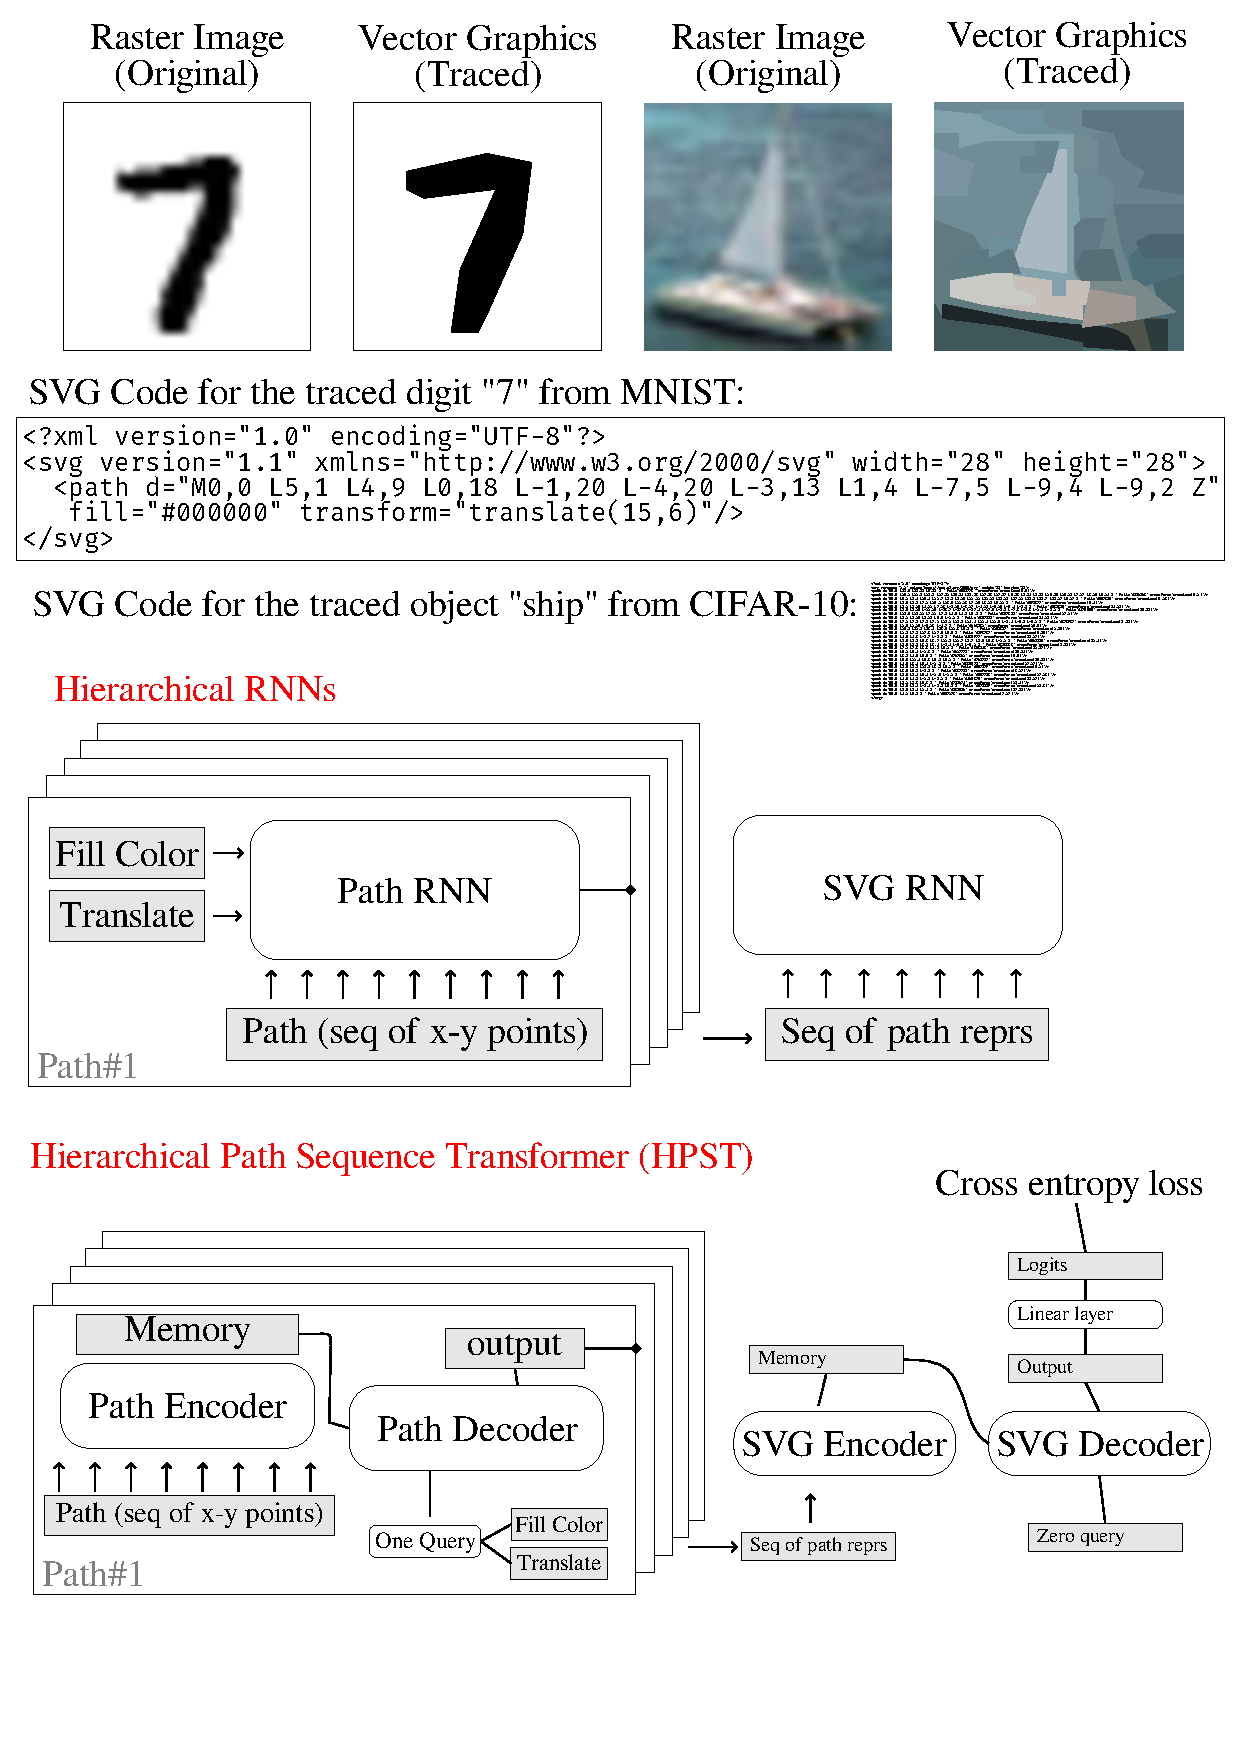
\includegraphics[width=1.0\linewidth]{demo.pdf}
    \caption{Demonstration}
\end{figure}

\textcolor{red}{Nobody has done this. But this is a more natural way to represent images in a sequence. 
And such sequence is approximate to human strokes.}

This will be novel enough as long as it works reasonably for MNIST, CIFAR-10,
CIFAR-100, Tiny-ImageNet, and ImageNet.

Reference: Image Vectorization: LIVE \cite{live,dvg}

In raster images representing textures as the first-order information,
the shapes as edges are stored as high-order information (computed from the
difference).
%
In contrast, in a vector image, both shape and texture are presented meanwhile
as the first-order information.
%
Namely, the polygon paths are directly shape information, while a combination of
a series of polygons in different colors form a texture (although the texture
may become coarse-grained if we want to limit the number of paths).

\section{Raster Graphics Vectorization}

Raster Graphics.

Raster Image Standard: PBM, BMP, JPEG, HEIF, etc.

Vector Graphics.

Vector Graphics standards: SVG.

Vector Image Rasterization.

Raster Image Vectorization. Bitmap Tracing (approximation)

\textcolor{red}{related: Primal sketches}

\textcolor{red}{stochastic grammar, songchun zhu, and/or graph}

\section{Our Approach}

(preliminary design)

hierarchical transformer.

path transformer for path representation. input is paths, sequence of points. init vector is color.

image transformer for image represetnation. input is sequence of paths.

\section{Experiments}

\subsection{Discussion on Vectorization Methods}

(1) \verb|inkscape| bitmap trace is very basic. It leverages some traditional
edge information from the image but the edges are not well seperated among
objects.

(2) \verb|vtracer| performs perfectly on MNIST, but for complicated images, it
creates too many paths. For instance, a daisy image from ImageNet leads to more
than $1000$ paths.  Training with such long nested sequences is expectedly very
difficult.

(3) LIVE~\cite{live} image vectorization.

(4) DiffVG~\cite{dvg} painterly rendering?

\subsection{Classification Performance}

GRU and HGRU works for both mnist and cifar

\begin{verbatim}
Dataset       Model     Accuracy  Parameters
============================================
MNIST         LeNet     98.9      431k
--------------------------------------------
MNIST         RNN       96.43     34k
..            GRU       97.31     84k
..            LSTM      96.89     109k
..            PST       97.30     211k
--------------------------------------------
MNIST         HRNN      96.66     59k
..            HGRU      98.00     159k
..            HLSTM     97.24     209k
..            HPST      98.17     412k
--------------------------------------------
FashionMNIST  LeNet     88.9      431k
--------------------------------------------
FashionMNIST  RNN       65.97     34k
..            GRU       72.88     84k
..            LSTM      72.08     109k
..            PST       72.19     412k
--------------------------------------------
FashionMNIST  HRNN      78.66     59k
..            HGRU      83.96     159k
..            HLSTM     82.79     209k
..            HPST      85.57     412k
--------------------------------------------
CIFAR10       ResNet18            11.6m
--------------------------------------------
CIFAR10       HRNN                59k
..            HGRU      55.21     159k
..            HLSTM               209k
..            HPST      68.78     412k
============================================
CIFAR10       (DDP 8 : RTX A6000)
              HRNN      33.08     59k
              HGRU      37.73     159k
              HGRU      43.24     828k (hidden_size 128, num_layers 4)
              HLSTM     31.82     209k
              HPST      53.06     412k
              HPST                1.6m (hidden_size 128)
============================================
\end{verbatim}


%%%%%%%%% REFERENCES
{\small
\bibliographystyle{ieee_fullname}
\bibliography{egbib}
}

\end{document}
